%!TEX root = ../thesis_a4.tex

\chapter{Background}
\label{chap:background}

\section{Introduction}

In this chapter we provide the relevant music and scientific background for the work presented in this dissertation. We start with a brief discussion on the terminology used in this thesis (\secref{sec:background_terminology}). Subsequently, we provide an overview of the selected music concepts relevant to better understand our work (\secref{sec:music_background}). We then present a review of the literature related with the topics addressed in this thesis. We first present relevant work done in computational analysis of \gls{iam} (SEction XX), which includes approaches for tonic identification, automatic \gls{raga} recognition and melodic pattern processing. Then, we present work done for other music traditions within \gls{mir} on topics covering melodic pattern processing and key recognition (\secref{sec:background_relevant_work_other_music}). Finally, we provide an overview of the select scientific concepts in information retrieval, time-series analysis, complex networks and statistics (\secref{sec:background_scientific_background}). We conclude this chapter by providing a summary of the literature review, wherein we highlight the shortcomings of the existing approaches, and identify some possible venues for scientific contribution (\secref{sec:background_summary}). 

\section{Terminology}
\label{sec:background_terminology}

In this section we provide working definition of the selected terms we have used throughout the thesis. Since the thesis focuses on the melodic description of \gls{iam}, it is important to clearly understand the meaning of melody in the context of this thesis. Our aim here is not to formally define melody in an universal sense, which as we see from the literature has been a challenge in itself, with almost every definition falling short of considering some aspect or the other XXXX. It would not be an overstatement to say that there is no agreed definition of melody that suits every context. For a review of interesting definitions of melody we refer to XXXX. Before we present the definition of melody that we consider in this work, it is important to understand the performance or concert setup in \gls{iam}. Since this music tradition is performance-based, even the studio recordings follow the same setup. Performances in \gls{iam} have a clearly defined concept of a lead artist, who plays the central role (also literally positioned in the center of the stage) and all other instruments are considered the accompaniments. In this context, mergin relevant parts of the definitions given by~\cite{paiva2006melody,kim2000analysis,levitin2002memory} covers to a large extent the scope of melody in \gls{iam}. Their definitions in the respective order are: \textquote{``\textit{the dominant individual pitched line in a musical ensemble}''} and \textquote{``\textit{an auditory object that emerges from a series of transformations along the six dimensions: pitch, tempo, timbre, loudness, spatial location, and reverberant environment}''}.  The first definition falls short of considering several other dimensions of sound such as timbre and loudness that are important in perception and production of melody, which are taken into account in the second definition. The concept of audio as a mixture of sounds from multiple instruments (`\textit{ensemble}') is missing in the second definition, which the first definition takes into account. The idea of continuity and smoothness of melody is expressed by `\textit{line}' in the former and by `\textit{series of transformations}' in the latter. If we combine these two definitions we can rewrite our working definition as \textquote{``\textit{an auditory object that emerges from a continuous series of transformations along the six dimensions: pitch, tempo, timbre, loudness, spatial location, and reverberant environment, by the dominant individual sound source in a music ensemble}''}. Although, we only consider the pitch dimension of melody in this thesis. Thus, loosely speaking, for all practical purposes within the scope of this thesis, we represent melody by a continuous pitch time-series corresponding to the lead artist in an audio recording, also referred to as predominant pitch in the subsequent chapters. This definition does not explicitly take into account the rare case of two lead artists. Since in a majority of such cases the two lead sound sources are active sequentially in time, our definition encompasses this scenario by considering the active sound source as dominant. \TODO{please make this shit better, these thigns are so confusing and broad}

Now that we have a working definition of melody, we proceed to define the scope of the terms such as melodic patterns, phrases and motifs in this thesis, and disambiguate them with other seemingly synonymous terms such as melodic fragment and segment. Melodic fragment or melodic segment in this thesis refers to a continuous subsequence of the pitch sequence. It does not entail any musical relevance in terms of the boundaries or the length of the subsequence. By a melodic pattern we refer to a repeating melodic fragment, where the scope and the meaning of repetition is based on the perceived melodic similarity. Across repetitions, a melodic fragment can undergo a series of time and pitch transformations allowed within the periphery of melodic framework (\gls{raga} in our case) without altering the identity of the melodic unit. Also, the melodic similarity here refers to the perceived similarity between melodic fragments when heard in isolation, as the local melodic context can influence the perception of similarity. Melodic patterns in this thesis do not entail any particular musical significance in terms them being characteristic of a melodic concept in \gls{iam}. The terms melodic pattens, fragments and segments are more from the perspective of signal or the time-series. Melodic phrases on the other hand are used in the context of music, as being a unit of melody which encapsulate an idea or a musical thought by an artist. Melodic motif is further high-level concept and we use it to refer to a particular type of characteristic patterns, in out thesis of \glspl{raga}, \gls{raga} motifs. 


The word polyphonic in the context of audio recordings signifies that the recordings consists of a mixtue of multiple instruments playing simultaneously.


\section{Music Background}
\label{sec:music_background}

\subsection{Indian Art Music}

\subsection{Melodies in Indian Art Music}

\subsubsection{Tonic in Indian art music}
\label{sec:background_tonic_in_iam}

\subsubsection{Svaras}

\subsubsection{Aroh-Avroh}

\subsubsection{Gamakas and Ornaments}

\subsubsection{Raga in Indian Art Music}

\paragraph{Phase-based and Scale-based ragas}
\paragraph{Allied ragas}

\subsubsection{Characteristic Melodic Phrases}

\subsubsection{Chalan}

\subsubsection{Nyas}
\label{sec:backgroung_nyas_description}

Dey presents various interpretations and perspectives on the concept of ny\={a}s in Hindustani music according to ancient, medieval and modern authors~\cite{Dey2008}. In the context of its current form, the author describes ny\={a}s as that process in a performance of a r\={a}g where an artist pauses on a particular \gls{svara}\footnote{The seven solf\`{e}ge symbols used in Indian art music are termed as \glspl{svara}. It is analogous to note in western music but conceptually different.}, in order to build and subsequently sustain the format of a r\={a}g, the melodic framework in Indian art music~\cite[p. 70]{Dey2008}\cite{KKG_SS13}. Dey elaborates the concept of ny\={a}s in terms of action, subject, medium, purpose and effect associated with it. Typically, occurrence of a ny\={a}s delimits melodic phrases (motifs), which constitute one of the most important characteristic of a r\={a}g. Analysis of ny\={a}s is thus a crucial step towards melodic analysis of Hindustani music. In particular, automatically detecting occurrences of ny\={a}s (from now on referred as ny\={a}s segments) will aid in computational analyses such as melody segmentation, motif discovery, r\={a}g recognition and music transcription~\cite{GopalJNMR2012, Rao2014}. However, detection of ny\={a}s segments is a challenging computational task, as the prescriptive definition of ny\={a}s is very broad, and there are no fixed set of explicit rules to quantify this concept~\cite[p. 73]{Dey2008}. It is through rigorous practice that a seasoned artist acquires perfection in the usage of ny\={a}s, complying to the r\={a}g grammar and exploring creativity through improvisation at the same time. 

\subsubsection{Recurring Melodic Patterns in IAM}


\section{Relevant Work in Indian Art Music}
\label{sec:background_relevant_work_iam}


\subsection{Tonic Identification}
\label{sec:background_relevant_work_tonic_identification}

In this section we provide a detailed review of the existing methods for tonic identification in audio recordings of \gls{iam}. The main objective of this review is to break down the methodology used across methods into a common set of processing blocks, and subsequently analyze different methods in terms of these blocks. Since in this thesis we also perform an extensive comparative evaluation of a number of these methods (\secref{sec:data_preprocessing_tonic_identification}), we review the methods in detail. In order to better interpret the output of these methods and to relate them with the processing steps and parameter choices, we provide the necessary implementation details, wherever required.


Identification of tonic pitch of the lead artist in an audio recording is a crucial first step in tonal analysis of \gls{iam} (\secref{sec:background_tonic_in_iam}). Knowing the tonic pitch used in an audio recording enables a meaningful comparison of melodies across different artists and their recordings. In this section we review existing approaches for automatic tonic identification in audio collections of \gls{iam}. 

As mentioned, there have been various efforts to automatically identify the tonic pitch of the lead artist in a performance of Indian art music~\citep{salamon2012multipitch,gulati2012two,bellur2012knowledge,ranjani2011carnatic,Sengupta2005b}. These approaches mainly differ in terms of the musical cues that they utilize to identify the tonic, the amount of input audio data used to perform this task and the type of music material they are devised for (Hindustani or Carnatic, vocal or
instrumental, etc.). Despite the differences, all these approaches can be divided into three main processing blocks, as shown in~\figref{fig:tonic_identification_general_block_diagram}. The only exception to this schema is the approach proposed by~\cite{Sengupta2005b}.

\begin{figure}
	\begin{center}
		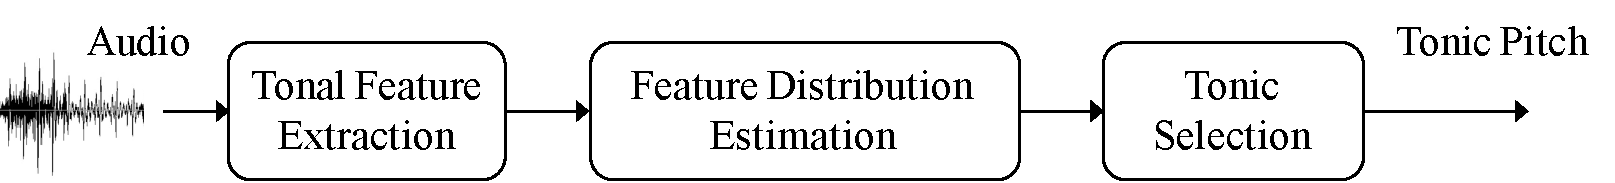
\includegraphics[width=\figSizeNinety]{ch02_background/figures/tonic_identification_block_diagram.pdf}
	\end{center}
	\caption[General block diagram of the processing steps used by tonic identification
	approaches.]{General block diagram of the processing steps used by tonic identification
		approaches.}
	\label{fig:tonic_identification_general_block_diagram}
\end{figure}


In all the aforementioned approaches, the three main processing blocks are the following: feature extraction, feature distribution estimation and tonic selection. Since the task of tonic identification involves an analysis of the tonal content of the audio signal, the features extracted in the first block are always pitch related. In the second block, an estimate of the distribution of these features is obtained using either Parzen window based density estimation or by constructing a histogram. The feature distribution is then used in the third block to identify the tonic. The peaks of the distribution correspond to the most salient pitch values used in the performance (usually the \glspl{svara} of the \gls{raga}), one of which corresponds to the tonic pitch. As the most salient peak in the distribution is not guaranteed to be the tonic, various techniques are applied to select the peak that corresponds to the tonic.

{\renewcommand{\arraystretch}{1.5}
	\begin{sidewaystable} 
		\begin{centering}
			\begin{tabular}{ c c c c }
				\tabletop			
				Method 	&	Features	&	Feature Distribution	&	Tonic Selection \\
				\tablemid			
				\acrshort{tonicid_sengupta} \citep{Sengupta2005b}	&	Pitch \citep{AKDatta_1996} & N/A & Error minimization\\
				
				\acrshort{tonicid_ranjani_1}/\acrshort{tonicid_ranjani_2} \citep{ranjani2011carnatic}	&	Pitch \citep{BoersmaPaul2001} & Parzen-window-based \acrshort{pde}  & GMM fitting\\
				
				\acrshort{tonicid_justin} \citep{salamon2012multipitch} & Multi-pitch salience \citep{Salamon2011} & Multi-pitch histogram & Decision tree\\
				
				\acrshort{tonicid_sankalp} \citep{gulati2012two}	& Multi-pitch salience  \citep{Salamon2011} & Multi-pitch histogram & Decision tree\\
				
				&	Predominant melody \citep{Salamon2012} & Pitch histogram & Decision tree\\
				
				\acrshort{tonicid_ashwin_1} \citep{bellur2012knowledge}	&	Pitch \citep{DeCheveigne2002}	&  \acrshort{gd} histogram & Highest peak\\
				
				\acrshort{tonicid_ashwin_2} \citep{bellur2012knowledge}	&	Pitch \citep{DeCheveigne2002}	& 	GD histogram	&
				Template matching\\
				
				\acrshort{tonicid_ashwin_2} \citep{bellur2012knowledge}	&	Pitch \citep{DeCheveigne2002}	& 	GD histogram
				& Highest peak\\
				
				\acrshort{tonicid_chordia}	& 	& 	& \\			
				
				\tablebot			
			\end{tabular}
			
			\caption[Summary of existing tonic identification approaches.]{Summary of existing tonic identification approaches.}
			\label{tab:pre_processing_tonic_identification_summary_methods}
			\par \end{centering}	
	\end{sidewaystable}
	
	
In \tabref{tab:pre_processing_tonic_identification_summary_methods} we provide a summary of the existing methods for tonic identification. The common processing blocks and the main differences between them become evident from this table. A detailed review of these methods in terms of the three processing stages as shown in \figref{fig:tonic_identification_general_block_diagram} is done in~\cite{Gulati2014Tonic}. For a more detailed description of these methods we refer to their respective publications listed in Table \tabref{tab:pre_processing_tonic_identification_summary_methods}. 


\subsubsection{Tonal Feature Extraction}
\label{Feature Extraction}

In the tonal feature extraction block (\figref{fig:tonic_identification_general_block_diagram}), the algorithms extract pitch-related
features from the audio signal for further processing. With the exception of \cite{SalamonSankalp2012,SGulatiIstanbul2012}, all approaches use a single feature, the predominant pitch in the audio. Note that whilst pitch and fundamental frequency ($f_0$) are not the same (the former being a perceptual phenomenon and the latter a physical quantity), for the purpose of tonic identification the $f_0$ is considered a reliable representation of pitch. Unlike these approaches, Salamon \cite{SalamonSankalp2012} uses a multi-pitch salience feature in order to exploit the tonal information provided by the drone instrument. Finally, Gulati \cite{SGulatiIstanbul2012} uses both the multi-pitch salience feature and the predominant melody. 

We now provide an overview of the algorithms used by the different approaches mentioned above for extracting $f_0$ and multi-pitch salience from audio recordings. \cite{ranjani2011carnatic} use the Praat software\footnote{Version 5.3.} \cite{BoersmaPaul2001} to obtain the pitch contours. The software implements the algorithm by~\cite{boersma1993accurate}, which is primarily proposed for speech signals and has also been used for monophonic music recordings in the past. \cite{Ashwin_Istanbul2012} uses an \gls{amdf} based pitch estimation algorithm, YIN, proposed by~\cite{DeCheveigne2002}. YIN is mainly developed for speech signals. As~\cite{DeCheveigne2002} make a remark,  the algorithm is informally tested on music and yet to be evaluated on polyphonic music. However, YIN has been used in a number of studies in \gls{mir} for pitch estimation from polyphonic music signals REF. \cite{Sengupta2005b} use a method based on \gls{psa} proposed by~\cite{AKDatta_1996} for extracting the $f_0$. Subsequently, a steady state detection is applied to the pitch contours in order to consider only the steady note regions for the analysis. Only segments of the pitch contour with a steady-state duration of at least 60 ms are used. It should be noted that this study was carried out using solo vocal performances (monophonic audio), which were carefully recorded in a studio without any kind of accompaniment present in the audio.

One of the possible caveats of the aforementioned pitch (strictly speaking, $f_0$) estimation methods is that they are all designed for monophonic signals containing a single sound source. This means that the number of estimation errors could increase as we add more instruments into the mixture. While due to the heterophonic nature of \gls{iam} and the prominent lead voice monophonic pitch trackers often manage to detect the $f_0$ of the lead artist even in the presence of accompaniment instruments. One way of overcoming this problem is by using a predominant pitch estimation algorithm. \cite{gulati2012two} use the method proposed by~\cite{Salamon2012} for estimating the pitch sequence of the predominant melody from the audio signal. \cite{gulati2012two} exploit the pitch information of the melody in the second stage of their approach to identify the specific octave of the tonic pitch (the tonic pitch-class is identified during the first stage of the algorithm).

As noted earlier, some recently proposed methods for tonic identification~\citep{salamon2012multipitch,gulati2012two} use a multi-pitch approach. Instead of extracting the predominant melodic component from the audio signal, the methods compute a multi-pitch time-frequency representation of pitch salience over time~\citep{Salamon2011}. The motivation for using multi-pitch analysis is twofold: first, as noted earlier, the music material under investigation is non-monophonic (includes many instruments playing simultaneously). Second, the tonic is continuously reinforced by the drone instrument, and this important cue can not be exploited by only extracting a single pitch value for each frame of the audio recording. To illustrate this point, in~\figref{fig:2HarmonicSeries} we display the spectrogram of a short audio excerpt of Hindustani music. Two types of harmonic series are clearly visible in the plot: the first consists of nearly straight lines and corresponds to the drone instrument (playing Sa and Pa). The second harmonic series (which start approximately at time 1 s) corresponds to the voice of the lead performer. Since the drone instrument is constantly present in the signal, a histogram of the peaks of the salience function will have prominent peaks at the pitches of the drone instrument, and this is exploited by \cite{SalamonSankalp2012,SGulatiIstanbul2012} for identifying the tonic. The main difference between the two approaches is that whilst~\citep{salamon2012multipitch} directly identifies the tonic pitch from the histogram, \cite{gulati2012two} divides the task into two stages: first the tonic pitch-class is identified using an extension of \cite{salamon2012multipitch}, and then the correct tonic octave is identified using the predominant melody information (see~\cite{Gulati2014Tonic} for further details).

\begin{figure}
	\begin{center}
		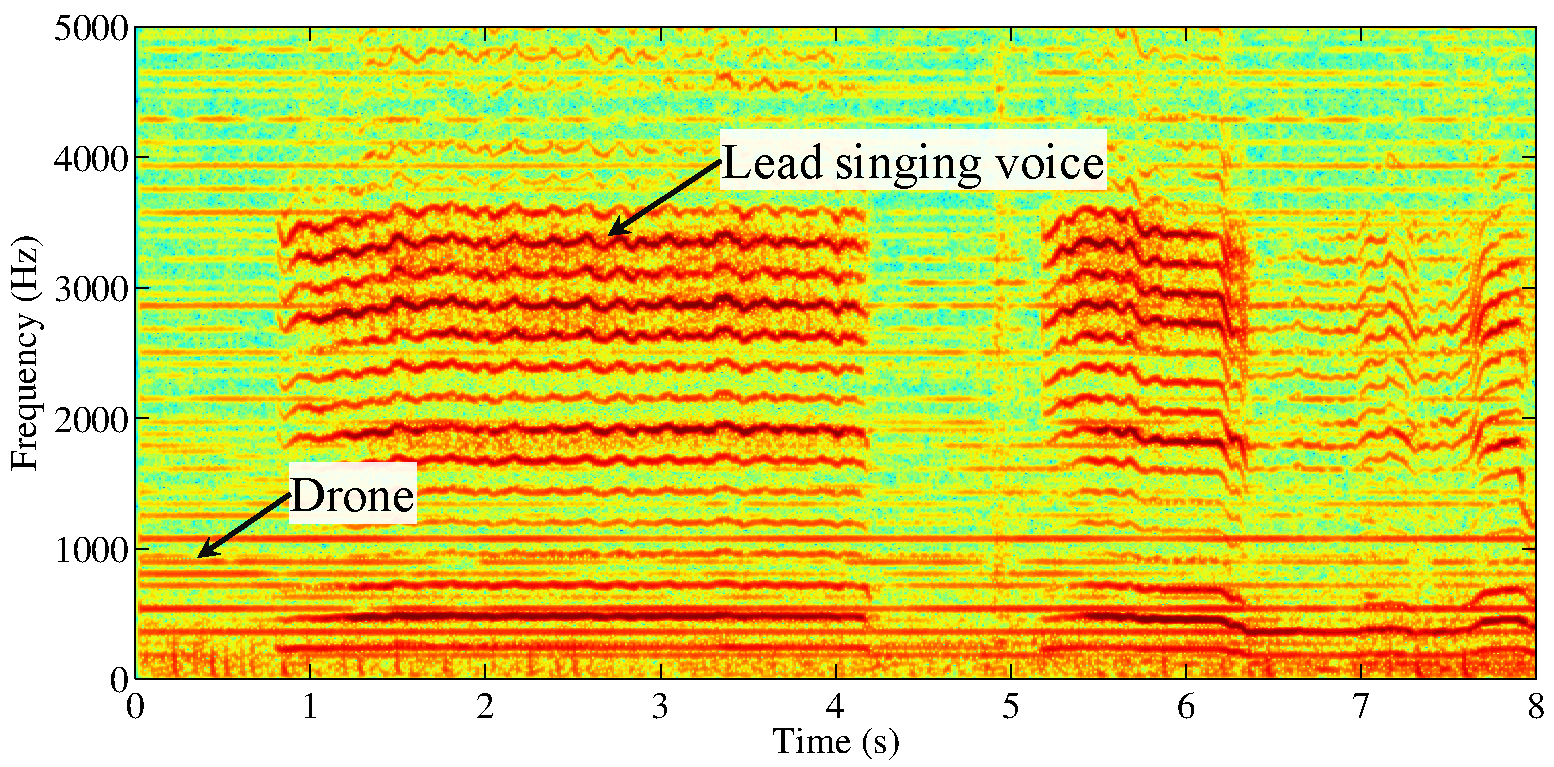
\includegraphics[width=\figSizeNinety]{ch02_background/figures/2HarmonicSeries.pdf}
	\end{center}
	\caption{Spectrogram of an excerpt of Hindustani music with two clearly visible types of harmonic series, one belonging to the drone and the other to the lead voice.}
	\label{fig:2HarmonicSeries}
\end{figure}


\subsubsection{Feature Distribution Estimation}
\label{sec:background_tonic_feature_distribution_estimation}

The tonal features extracted by the different tonic identification approaches are subsequently analyzed in a cumulative manner (cf.~block two in Figure \ref{fig:tonic_identification_general_block_diagram}). The pitch values from all analysis frames (whether a single value is computed per frame or multiple values) are aggregated into a pitch distribution function, which reflects the (possibly weighted) rate of occurrence of different pitch values in the entire audio excerpt. The peaks of the pitch distribution function represent the most frequent (or salient if weighting is used) pitches in the recording, one of which will be the tonic. The only exception is the approach proposed by~\cite{Sengupta2005b}, which instead of analyzing the distribution of the features, computes an aggregate error function in order to select the tonic. The methods used by the different tonic identification approaches for estimating the pitch distribution function are described below.

In~\cite{salamon2012multipitch,gulati2012two}, the pitch values of the peaks of the salience function in every frame are aggregated into a histogram. The top 10 peaks in every frame are used, in this way ensuring that in addition to the lead instrument/voice, the pitch content of other accompanying instruments is also captured, most importantly the notes played by the drone instrument. The frequency range considered for selecting the peaks of the salience function for constructing the histogram is restricted to 100-370 Hz (note that the typical frequency range for the tonic 100-260 Hz). The reason for computing the histogram beyond 260 Hz even though the tonic rarely goes above this frequency is that in some cases the aforementioned methods can exploit the presence of a peak corresponding to the fifth/fourth (Pa/Ma) above the tonic in order identify the tonic pitch. Since in many cases the lead voice/instrument is considerably louder than the drone sound, the weights of the salience peaks are ignored when computing the histogram, meaning only the rate of occurrence is taken into account. As noted earlier, the result is that the pitches produced by the drone instrument (the tonic and Pa, Ma or \gls{ni}) manifest in the form of high peaks in the histogram, since the drone sounds continually in the recording. The resulting pitch distribution thus depends heavily on the notes of the drone instrument. This would not be the case if we only considered the predominant melody for computing the histogram, in which case the pitch distribution would depend on the chosen \gls{raga}, thus increasing the complexity of identifying the tonic.

\begin{figure}
	\begin{center}
		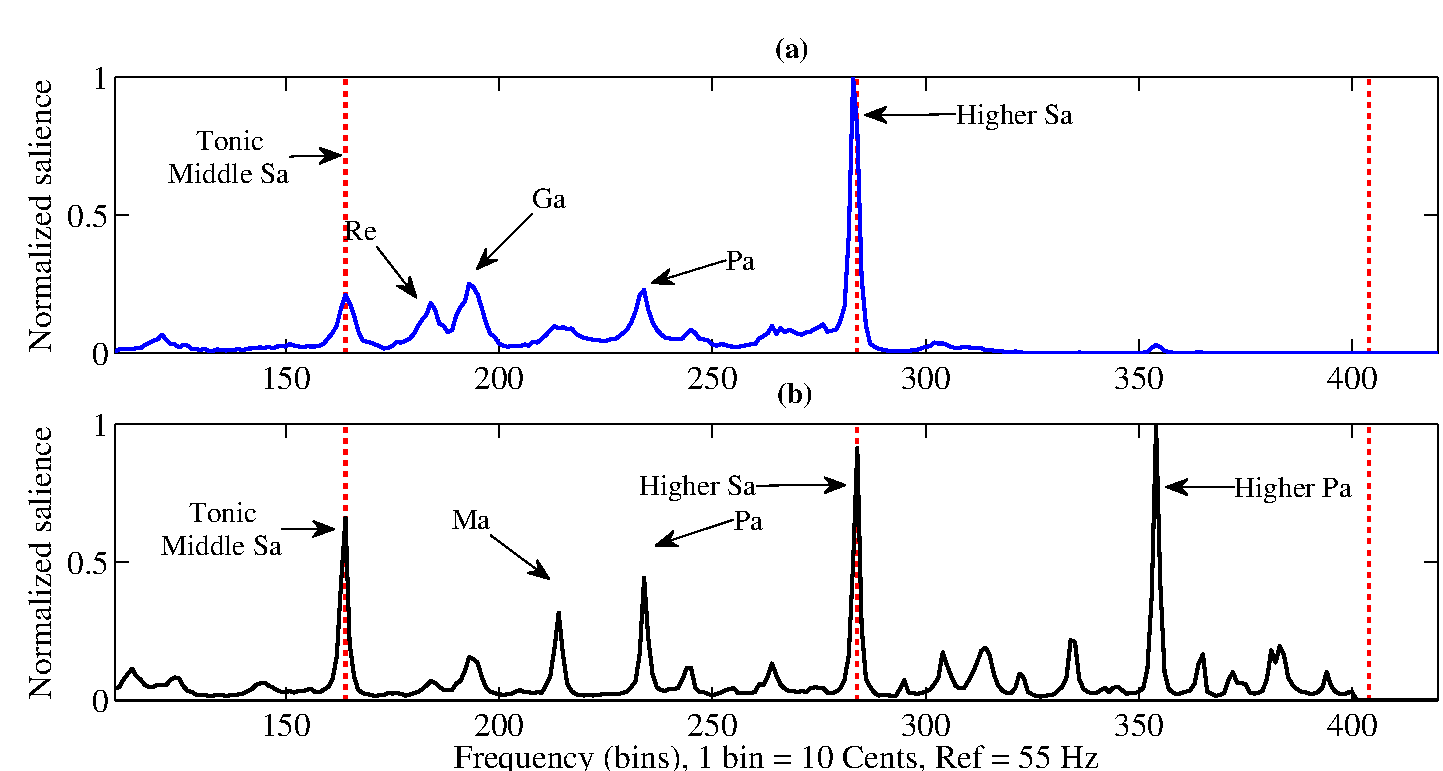
\includegraphics[width=\figSizeNinety]{ch02_background/figures/Histogram_Melody_Multipitch.pdf}
	\end{center}
	\caption[Comparison of the histograms constructed using different methods]{Pitch histograms for the same excerpt constructed using (a) predominant melody (in blue) and (b) peaks of a multi-pitch salience function (in black). The tonic pitch-class locations are indicated with red dotted lines.}
	\label{fig:background_pitch_histograms_multipitch}
\end{figure}

In Figure \ref{fig:background_pitch_histograms_multipitch} we display two pitch histograms, computed using (a) the pitch of the predominant melody and (b) the peaks of a multi-pitch salience function. Both histograms are computed from the same three-minute audio excerpt. We see that in the histogram computed using the predominant melody (a), the prominent peaks correspond to \glspl{svara} Sa, Ga and Re (the prominent \glspl{svara} of \gls{raga} \textit{Sindh Bhairav\={i}} ), whereas in the multi-pitch histogram (b), the top three peaks correspond to Sa (in two octaves) and Pa, which are the prominent \glspl{svara} produced by the drone instrument. 

In~\cite{Ashwin_Istanbul2012}, a histogram is constructed using a frequency range of 40-800 Hz with a 1 Hz resolution and later post processed using a group delay function. The authors show that by assuming that the constructed pitch histogram is the squared magnitude of resonators in parallel, group delay functions can be applied to obtain a better resolution for the peaks in the resulting histogram. It is also shown that a group delay function accentuates peaks with lesser bandwidths. Given that the \gls{shadja} (tonic pitch-class) and panchama (3/2 of the tonic pitch-class) in all octaves are relatively less inflected, this characteristic of the group delay function is shown to be beneficial for improving the accuracy of tonic identification. The processed histograms are referred to as \gls{gd} histograms.

\cite{Ashwin_Istanbul2012} also propose the concept of segmented histograms. In order to exploit the omnipresence of the \gls{shadja},  it is proposed that, given the pitch contour for an item of music, the contour is segmented into smaller units and a \gls{gd} histogram is constructed for each of these smaller units. Given that \gls{shadja} will be present in all the units, the peak corresponding to the \gls{shadja} will be enhanced in the corresponding \gls{gd} histograms. The individual histograms are then multiplied bin-wise. This also helps in reducing the height of the non \gls{shadja} peaks which might not be present in all the segments. Tonic selection is then performed on the resulting histogram, referred to as the segmented \gls{gd} histogram.

Instead of using a histogram, \cite{ranjani2011carnatic} use a Parzen window estimator to compute a pitch density function~\citep{Bishop,DudaHart2000}. Parzen window estimators (or kernel density estimators) are non-parametric density estimators. The choice of kernel function can control the smoothness of the estimated density. They are widely used as an alternative to histograms to alleviate the artificial discontinuities at the boundaries of the bins of the histogram, and aid in a smoother peak picking process. In addition, they do not require partitioning of data into distinct bins. \cite{ranjani2011carnatic} use parzen window estimators with Gaussian kernels for estimating the density of the extracted pitch frequencies.


\subsubsection{Tonic selection}
\label{Tonic Selection}

In the previous section we discussed different ways to compute the pitch distribution function. This section presents the last processing block shown in~\figref{fig:tonic_identification_general_block_diagram}, where the pitch distribution function is used to identify the tonic pitch. The peaks of the pitch distribution function correspond to the most frequent (or salient) pitches present in the audio signal. Depending on how the pitch distribution is computed the peaks will coincide with the \glspl{svara} of the \gls{raga} used in the rendition or with the \glspl{svara} produced by the drone instrument. The problem of tonic identification is thus reduced to selecting the peak of the distribution that corresponds to the tonic of the lead artist. As noted earlier, the peak corresponding to the tonic pitch is not always the highest peak in the distribution. For this reason, various strategies are have been proposed for analyzing the pitch distribution and selecting the peak that corresponds to the tonic. The complexity of the approaches varies from simply selecting the highest peak of the histogram to the application of machine learning algorithms in order to automatically learn the best set of rules for selecting the tonic peak. The different tonic selection strategies used in the literature are presented below.

\cite{Ranjani2011} model the pitch distribution using semi-continuous Gaussian mixtures~\cite{Huang2001}, motivated by the following two musical cues in Indian art music: first, the relative positions of the \glspl{svara} with respect to the tonic hover around a mean ratio \cite{Krishnaswamy2003} and second, the \gls{shadja} (tonic pitch-class) and panchama (fifth of the tonic pitch-class) are the prakrthi \glspl{svara} which means they are sung/played without any inflections \cite{Manikandan2004,Krishnaswamyicassp2003}. Peaks of the pitch density function within a suitable pitch range are selected as possible tonic candidates. The variance of the pitch distribution around the peaks is estimated by modeling each tonic candidate (i.e.~peak) with a Gaussian distribution. As noted above, one of the key characteristics of \gls{shadja} and panchama is that they do not vary (in pitch) throughout the performance. Thus, the parameters of the Gaussian model are used to infer the correct tonic candidate. The pitch range used for selecting tonic candidates is 100\,-\,250\,Hz. When the editorial metadata of the audio recording is known, the pitch range is further constrained depending on the gender of the lead artist. The range for male singers is set to 100\,-\,195 Hz and for female singers is set to 135\,-\,250 Hz.

\cite{salamon2012multipitch,gulati2012two} use a classification based approach to identify the peak of the multi-pitch histogram that corresponds to the tonic pitch \cite{salamon2012multipitch} or tonic pitch-class \cite{gulati2012two}. Since all the pitches in a performance are in relation to the tonic, the relationships between the peaks of the histogram (height and distance) are used to compute a set of features, which are then used to train a classifier for identifying which peak corresponds to the tonic. In this way, rather than having to manually define a template for selecting the tonic, an optimal set of rules are learned automatically using machine learning. The authors extract height and distance related features for the top 10 peaks in the multi-pitch histogram. The authors show that for the tonic identification task the C4.5 decision tree classifier~\cite{Quinlan:1993:CPM:152181} yields the highest classification accuracy. 

\cite{SGulatiIstanbul2012} uses a similar classification-based approach to first identify the peak of the histogram that corresponds to the tonic pitch-class. The correct tonic octave is then determined in the second stage of processing, which is also classification-based. For every candidate tonic pitch (candidates have the same pitch class but are in
different octaves) a set of 25 features is computed. The features are the values of the melody histogram at 25 equally spaced locations spanning two octaves centered around the tonic pitch candidate. The classification is a two-class problem: either the pitch candidate is in the correct octave, or it is not. As done in~\cite{salamon2012multipitch}, a C4.5 decision tree is trained using the Weka data-mining software for the classification. For a detailed description of the method we refer to~\cite{SGulati_MThesis2012}.

\cite{Sengupta2005b} use an error minimization technique to identify the tonic. This is a brute force approach: a large number of pitch values within a pre-defined frequency range are considered as candidates for the tonic pitch. A cumulative deviation is computed between the steady state regions of the pitch contour (described in~\secref{sec:background_tonic_feature_distribution_estimation}) and the pitch values of the closest notes to these regions, which are obtained using three different tuning schemas given a tonic candidate. The tonic candidate which results in the minimum deviation is selected as the tonic of the musical excerpt.

\cite{Ashwin_Istanbul2012} propose a simple approach, picking the highest peak of the pitch distribution as the tonic. In two out of the three proposed variants of their method, the bin value of the highest peak of the segmented \gls{gd} pitch histogram is selected as the tonic pitch. The frequency range of the histogram is restricted to 100-250\,Hz. When the gender information of the lead artist for an audio recording is available, this range is further restricted. In addition to the simple highest peak approach, \cite{Ashwin_Istanbul2012} also propose a template matching process to identify tonic. This procedure is comparable to the Semi-continuous GMM fitting proposed by \cite{Ranjani2011}, which exploits the smaller degree of pitch variation around \gls{shadja} and panchama. The template that authors use to identify the tonic candidate uses three octaves and consider the pitch distribution values at tonic and its fifth (Pa) in different octaves. For more information we refer to~\cite{Gulati2014Tonic}.


\TODO{A concluding paragraph of this section, motivating the need for a thorough evaluation.}


\subsection{\Glsentrytext{raga} Recognition}
\label{sec:sota_raga_recognition}


\begin{sidewaystable}
	\begin{threeparttable} 
		\ra{1.1}
		\setlength{\tabcolsep}{2pt}
		\small
		\begin{centering}
			\begin{tabular}{l L{2.5cm} L{2cm} L{2.5cm} L{2.5cm} L{2.5cm} L{2.5cm} L{2.5cm}}
				\tabletop
				& Svara set & Svara salience & Svara intonation & \Gls{arohana}-\gls{avrohana} & Melodic phrases & Svara discretization & Temporal aspects\tabularnewline
				\tablemid
				\cite{pandey2003tansen} &  &  &  & $\bullet$ & $\bullet$ & Yes & $\bullet$\tabularnewline
				\cite{chordia2007raag} & $\bullet$ & $\bullet$ &  & $\bullet$ &  & Yes & $\bullet$\tabularnewline
				\cite{belle2009raga} & $\bullet$ & $\bullet$ & $\bullet$ &  &  & No & \tabularnewline
				\cite{Shetty2009} & $\bullet$ &  &  & $\bullet$ &  & Yes & $\bullet$\tabularnewline
				\cite{sridhar2009raga} & $\bullet$ &  &  & $\bullet$ &  & Yes & $\bullet$\tabularnewline
				\cite{koduri2011survey} & $\bullet$ & $\bullet$ &  &  &  & Yes & \tabularnewline
				\cite{ranjani2011carnatic} & $\bullet$ &  &  &  &  & No & \tabularnewline
				\cite{chakraborty2012object} & $\bullet$ &  &  &  &  & Yes & \tabularnewline
				\cite{koduri2012raga} & $\bullet$ & $\bullet$ & $\bullet$ &  &  & Both & \tabularnewline
				\cite{chordia2013joint} & $\bullet$ & $\bullet$ & $\bullet$ &  &  & No & \tabularnewline
				\cite{dighe2013scale} & $\bullet$ & $\bullet$ &  & $\bullet$ &  & Yes & $\bullet$\tabularnewline
				\cite{dighe2013swara} & $\bullet$ & $\bullet$ &  &  &  & Yes & \tabularnewline
				\cite{koduri2014intonation} & $\bullet$ & $\bullet$ & $\bullet$ &  &  & No & \tabularnewline
				\cite{kumar2014identifying} & $\bullet$ & $\bullet$ & $\bullet$ & $\bullet$ &  & Yes & $\bullet$\tabularnewline
				\cite{shrey_ISMIR_2015}\tnote{a} &  &  &  &  & $\bullet$ & No & $\bullet$\tabularnewline	
				\tablebot
			\end{tabular}
			\par \end{centering}
		
		\begin{tablenotes}
			\item[a] This method performs \gls{raga} verification and not recognition
		\end{tablenotes}
		\caption{\Gls{raga} recognition methods proposed in the literature along with the melodic characteristics they utilize to perform the task. We also indicate if a method uses a discrete \gls{svara} representation of melody. The methods are arranged in the chronological order. \TODO{review the approaches and verify}}
		\label{tab:raga_recognition_methods_melodic_characteristics}
	\end{threeparttable}
\end{sidewaystable}


\begin{sidewaystable}
	\begin{threeparttable} 
		\tiny
		\ra{1.1}
		\begin{centering}
			\begin{tabular}{l l P{2cm} P{3cm} P{2.5cm} L{1cm} P{1.5cm} P{2cm}}
				\hline 
				& \textbf{Tonal Feature} & \textbf{Tonic } & \textbf{Feature} & \textbf{Recognition Method} & \textbf{\#Ragas} & \textbf{Dataset Size (Dur./Num)}\tnote{i} & \textbf{Audio Type}\tabularnewline
				\hline 
				\cite{pandey2003tansen} & \cite{BoersmaPaul2001}\tnote{p} & Fixed frequency & Svara sequence & \acrshort{hmm} and \acrshort{ngram} & 2 & NA / 31 & Monophonic\tabularnewline
				\cite{chordia2007raag} & \cite{sun2000pitch}\tnote{p} & Manual & PCD, PCDD & \acrshort{svm} classifier & 31 & 20 / 127 & Monophonic\tabularnewline
				\cite{belle2009raga} & \cite{rao2009improving}\tnote{p} & Manual & PD (parameterized) & \acrshort{knn} classifier & 4 & 0.6 / 10 & Polyphonic\tabularnewline
				\cite{Shetty2009} & \cite{sridhar_2006_svara}\tnote{p} & Fixed frequency & \#Svaras, its combinations, Vakra svaras & Neural Network classifier & 20 & NA / 90 & Monophonic\tabularnewline
				\cite{sridhar2009raga} & \cite{lee2006automatic}\tnote{p} & Singer identification & Svara set, its sequence & String matching & 3 & NA / 30 & Polyphonic\tabularnewline
				\cite{koduri2011survey} & \cite{rao2010vocal}\tnote{p} & Brute force & PCD & \acrshort{knn} classifier & 10 & 2.82 / 170 & Polypohonic\tabularnewline
				\cite{ranjani2011carnatic} & \cite{BoersmaPaul2001}\tnote{p} & GMM fitting & PDE & SC-GMM and Set matching & 7 & NA / 48 & Polyphonic\tabularnewline
				\cite{chakraborty2012object} & \cite{sengupta1990study}\tnote{p} & Error minimization & Svara set & Set matching & NA & NA / NA & NA\tabularnewline
				\cite{koduri2012raga} & \cite{Salamon2012}\tnote{p} & Multipitch-based & PCD variants & \acrshort{knn} classifier & 43 & NA / 215 & Polyphonic\tabularnewline
				\cite{chordia2013joint} & \cite{camacho2007swipe}\tnote{p} & Brute force & PCD variants & \acrshort{knn} and statistical classifiers & 31 & 20 / 127 & Monophonic\tabularnewline
				\cite{dighe2013scale} & Chroma~\citep{lartillot2008matlab}\tnote{c} & Brute force (Vadi-based) & Chroma, Timbre features & \acrshort{hmm}  & 4 & 9.33 / 56 & Polyphonic\tabularnewline
				\cite{dighe2013swara} & \citep{lartillot2008matlab}\tnote{c} & Brute force (Vadi-based) & PCD variant & Random Forest & 8 & 16.8 / 117 & Polyphonic\tabularnewline
				\cite{koduri2014intonation} & \cite{Salamon2012}\tnote{p} & Multipitch-based & PCD (parameterized)  & Several classifiers & ?? & ?? & Polyphonic\tabularnewline
				\cite{kumar2014identifying} & \cite{Salamon2012}\tnote{p} & Brute force & PCD + \acrshort{ngram} distribution & \acrshort{svm} classifier  & 10 & 2.82 / 170 & Polyphonic\tabularnewline
				\cite{shrey_ISMIR_2015}{*} & \cite{Salamon2012}\tnote{p} & Cepstrum-based & Pitch contours & LCSS with \acrshort{knn} & 30 & 3 / 254 & Polyophonic\tabularnewline
				\hline 
			\end{tabular}
			\par \end{centering}
		\begin{tablenotes}
			\item[i] In the case of multiple datasets we list the larger one
			\item[p] Pitch extraction algorithm
			\item[c] Chroma extraction algorithm
			\item[*] This method performs \gls{raga} verification and not recognition
		\end{tablenotes}
		\caption{Summary of the \Gls{raga} recognition methods proposed in the literature. The methods are arranged in the chronological order. \TODO{review the approaches and verify. Put specific resolution of PCD and mark if they used KDE based PCD? also make it consistent the vocabulary. Clean it further and use more meaningful descriptor names. Both Dighe paper use chroma feature...chromagram types...not PCD variant. Verify all these details..}}
		\label{tab:raga_recognition_methods_details}
	\end{threeparttable}
\end{sidewaystable}

In this section we present a critical review of the existing computational approaches for \gls{raga} recognition in audio collections of \gls{iam}. Our main objective in this review is to consolidate existing work on automatic \gls{raga} recognition, identify the strengths and shortcomings of different methodologies, and finally, identify potential venues of improvement. The accuracy of a \gls{raga} recognition system largely depends on the size of the dataset in terms of the number of \glspl{raga} and also on the chosen set of \glspl{raga}. The task becomes even more challenging when the chosen set of \glspl{raga} in the dataset share a common set of \glspl{svara} and are allied \glspl{raga} (Section XX). Since the approaches reviewed in this section are evaluated on different datasets (typically collected for a single study, and is not publicly made available), we refrain from comparing absolute \gls{raga} recognition accuracies across studies. 

We now proceed to review the existing \gls{raga} recognition approaches. Due to the central role of the \gls{raga} framework in \gls{iam}, its automatic identification is one of the most researched topics in computational analysis of this music tradition. Over the last couple of decades there have been several approaches proposed for this task. In \tabref{tab:raga_recognition_methods_melodic_characteristics} and \tabref{tab:raga_recognition_methods_details} we summarize the prominent existing approaches for \gls{raga} recognition. Both the tables comprise exactly the same set of approaches, but differ in terms of the type of information provided for each approach. In \tabref{tab:raga_recognition_methods_melodic_characteristics} we indicate the different characteristic features of a \gls{raga} that these approaches exploit to perform the task. The melodic attributes that we have considered to summarize the approaches are; \gls{svara} set, \gls{svara} salience, \gls{svara} intonation, \gls{arohana}-\gls{avrohana} and melodic phrases. In addition to these melodic attributes, we also mark if an approach uses a discretized melodic representation, and if it considers the temporal aspects of the melody to perform the task. In \tabref{tab:raga_recognition_methods_details} we provide the relevant details for each approach in terms of the common processing blocks such as the feature extraction, the tonic identification, the learning method used to recognize \glspl{raga} and the other relevant dataset details. With both these tables we get an bird's-eye view of the existing work done in \gls{raga} recognition.

From \tabref{tab:raga_recognition_methods_melodic_characteristics} we see that the most frequently used melodic attribute is the set of \glspl{svara} in a \gls{raga}, which is also computationally one of the most basic feature to extract. \Gls{svara} set is considered as a feature for \gls{raga} recognition in a both explicit and implicit manner by different approaches. \citep{chakraborty2012object,ranjani2011carnatic} explicitly extract the comprising set of \glspl{svara} in an audio recording. The \gls{raga} of the recording is then identified by matching the estimated \gls{svara} set with the stored set for each \gls{raga}. The exact procedure followed to map the estimated \gls{svara} set with a unique \gls{raga} label is missing in the articles. As can be imagined, it is a rather naive approach since there are several \glspl{raga} that share the same set of \glspl{svara} and are differentiated based on more elaborate melodic and temporal characteristics.

Along with the set of \glspl{svara}, \gls{raga} grammar also defines the functional roles of these \glspl{svara} (Section XX). In particular, there is a vocabulary to describe the salience of the \glspl{svara} in a melody such as \gls{vadi} and \gls{samvadi}. Thus, one of the ways to differentiate between the \glspl{raga} that share a common set of \glspl{svara} is to also consider the salience of the comprising \glspl{svara} in the analysis. Computing \gls{svara} salience for all the possible \glspl{svara} frequencies implicitly incorporates the \gls{svara} set feature. This is the reason why it appears for nearly all the approaches mentioned in \tabref{tab:raga_recognition_methods_melodic_characteristics}. \cite{chordia2007raag} propose a feature that jointly incorporates the presence and the salience of different \glspl{svara} in a melody for recognizing \glspl{raga}. The authors represent \gls{svara} saliences using a 12 bin \gls{pcd} computed as a histogram of the pitch sequence for an audio recording. This global feature is robust to pitch octave errors and is shown to perform well on a sizable dataset. The approach proposed by~\cite{chordia2007raag} for computing \gls{pcd} implicitly considers the duration of the \glspl{svara} in a melody for estimating their saliences. However, the meaning of the salience of a \gls{svara} in a melody is not explicitly defined in the music theory, and therefore, it can be interpreted and computed in multiple ways. \cite{koduri2011survey} explore two different approaches for computing \gls{pcd}, which differ in the way \gls{svara} salience is interpreted. One of the proposed approaches for computing \gls{pcd} weighs the salience by the duration of the \glspl{svara} as done in~\cite{chordia2007raag}. Whereas, the other approach considers the frequency of the occurrence of \glspl{svara} as the salience, irrespective of their duration. The former was reported to result in a better accuracy.

A simple extension to the 12 bin \gls{pcd} feature mentioned above is computing the pitch distribution using a fine grained bin boundaries. A high resolution \gls{pcd} in addition to the \gls{svara} saliences also captures the intonation aspects of the \glspl{svara}. Such a fine grained \gls{pcd} is used in~\cite{chordia2013joint,koduri2012raga,belle2009raga,kumar2014identifying}. These studies report a superior performance by using the high resolution \gls{pcd} as compared to a 12 bin \gls{pcd}. Note that in~\cite{chordia2013joint} the authors refer to the high resolution \gls{pcd} by \gls{fpd}. Apart from the high resolution \glspl{pcd}, there are other variants of the \gls{pcd} feature, wherein the technique used for computing the pitch distribution is based on the concept of \gls{kde}. Such a variant of the \gls{pcd} feature is used in~\cite{chordia2013joint,ranjani2011carnatic} and is reported to improve the \gls{raga} recognition accuracy. Note that these variants are referred to as \gls{kpd} in~\cite{chordia2013joint} and \gls{pde} in~\cite{ranjani2011carnatic}. 

The high resolution \gls{pcd} features mentioned above implicitly capture some of the intonation aspects of the \glspl{svara} in a melody. However, controlling the weight of the \gls{svara} intonation aspects in the \gls{pcd} feature space for \gls{raga} recognition is a challenging task. To address this issue, \cite{belle2009raga,koduri2014intonation} propose to use a parametrized version of the \gls{pcd}, wherein the parametrization is performed for each \glspl{svara} in the melody. \cite{belle2009raga} extract four different features for each \gls{svara}; peak position, mean position, variance and overall probability of the \gls{svara}.  In a similar manner, \cite{koduri2014intonation} extract six features for each \gls{svara}; peak position, peak amplitude, mean, variance, skewness and kurtosis of the \gls{svara} distribution. Melodies in Carnatic music contain \glspl{gamaka} (Section XX), during which the pitch deviation even in the rendition of a single \gls{svara} can reach up to 200\,cents. To capture the intonation aspects in such scenarios it is essential to identify which \gls{svara} is being rendered at a given point in time in a melody. For that, \cite{koduri2014intonation} also propose an alternate approach to compute context-based \gls{svara} distribution by categorizing pitch contours based on the melodic context. Subsequently, the parametrization to extract six features is performed on these context-based \gls{svara} distribution. \cite{koduri2014intonation} report that context-based \gls{svara} distribution obtain a better results in classifying \glspl{raga}.

One of the shortcomings of the approaches discussed so far is that they do not consider the temporal aspects of melody, which are fundamental in characterization of \glspl{raga}. There exist a number of approaches that statistically capture the temporal aspects of melody by modeling essentially the \gls{arohana}-\gls{avrohana} progression of the \glspl{raga}~\citep{pandey2003tansen,chordia2007raag,Shetty2009,sridhar2009raga,dighe2013scale,kumar2014identifying}. A number of these methods compute \gls{svara} sequence and employ techniques such as \gls{hmm} and \gls{ngram} to model the temporal aspects~\citep{pandey2003tansen,dighe2013scale,kumar2014identifying}. Some approaches compute an intermediate representation that captures the temporal aspects, such as \gls{pcdd} in~\cite{Pchordia2007raag} and \gls{svara} combination feature in~\cite{Shetty2009}, which are then fed to a classifier to learn the discriminatory model for different \glspl{raga}. Few of these approaches also utilize characteristic melodic phrases of \glspl{raga}~\citep{pandey2003tansen,sridhar2009raga}. They store a dictionary of pre-defined melodic patterns for each \gls{raga}, and subsequently detect the occurrences of these patterns in the \gls{svara} sequences obtained from the test recordings to recognize \glspl{raga}. The scalability of these approaches is however questionable, since they have been evaluated on a dataset comprising only two to three \glspl{raga}. 

The approaches mentioned above invariably consider a discrete representation of melody by either performing a simple quantization of the estimated pitch contours or by using a relatively sophisticated melodic transcription technique~\cite{pandey2003tansen}. Since melodic transcription still remains a challenging and an ill-defined task for melodies in \gls{iam}, this step introduces errors that further propagate and influence the final accuracy of the methods. Although, a formal quantitative evaluation of the influence of the errors introduced during the melody transcription stage on the final accuracy is yet to be performed. Apart from the challenges arising from the melody transcription stage, another limitation of the approaches mentioned above is that they fall short of capturing the relevant information in the melody transitions across the \glspl{svara}. Calan of a \gls{raga} outlines the way melody progresses from one \gls{svara} to another, and therefore, is a characteristic feature of a \gls{raga}. Such a fine grained temporal melodic aspects are considered in the approaches that use a continuous melodic representation and utilize melodic patterns for recognizing \glspl{raga}. Owing to the challenges involved in discovering and detecting patterns in continuous melody representation, there are not many approaches follow this methodology. \cite{shrey_ISMIR_2015} perform \gls{raga} verification using automatically discovered melodic patterns from specific sections (Pallavi lines) of audio recordings in Carnatic music. A \gls{raga} verification system as opposed to a recognition system assumes that a specific \gls{raga} is claimed and the system checks whether the claimed \gls{raga} is correct or not. Thus, \gls{raga} verification can be regarded as a subset of \gls{raga} recognition with a reduced complexity of the task. 

With the exception of the methods proposed by~\cite{dighe2013scale,dighe2013swara} all other methods use pitch as the tonal feature for performing \gls{raga} recognition (\tabref{tab:raga_recognition_methods_details}). These methods employ a variety of pitch estimation algorithms. While some of these pitch estimation algorithms are specifically designed to work with polyphonic audio music content~\cite{Salamon2012}, others are primarily suitable for monophonic speech signals~\cite{BoersmaPaul2001}. Thus, incorrect estimation of the pitch from the audio signals might be a potential source of errors in the system. However, since some of these methods are evaluated using monophonic audio music content and the others with polyphonic content, it is hard to make that conclusion from the results reported in the studies. Verification of this hypothesis remains up to a comprehensive comparative evaluation on a common dataset. As mentioned, the exceptions to using the pitch feature for \gls{raga} recognition are the methods proposed by \cite{dighe2013scale,dighe2013swara}, which use a 12 bin chroma feature to perform the task. Chrome feature has been widely used for key and mode identification task~\TODO{ref}. The computation of chroma features considers all the tonal components in the audio music signal. In the case of \gls{iam} that would imply considering the \gls{tabla} and the \gls{tanpura} sound, which is often in the background and reinforce the base \gls{svara} Sa. Thus, considering the tonal components that are not at all related to the underlying \gls{raga} can degrade the performance of the method. However, since none of the studies~\citep{dighe2013scale,dighe2013swara} compare the performance with a pitch feature based \gls{raga} recognition system, no conclusion can be drawn without a comparative evaluation \TODO{double check this point}.

A crucial step in \gls{raga} recognition is making the method invariant to the tonic pitch of the lead artist used in an audio recording. As seen in~\tabref{tab:raga_recognition_methods_details}, there are multiple ways this is addressed by the existing approaches. A number of these studies either perform a tonic normalization by manually estimating the tonic pitch of the lead artist in the recording, or they only consider performances in a fixed pre-defined tonic pitch~\citep{pandey2003tansen,chordia2007raag,belle2009raga,Shetty2009}. In either case these methods are not scalable to real-world collections, where the tonic pitch varies across artists and recordings, and manually extracting this information can be a cumbersome task. To alleviate this limitation, several methods either employ an external automatic tonic identification module~\citep{koduri2012raga,koduri2014intonation} or they explicitly identify tonic pitch prior to \gls{raga} recognition~\citep{ranjani2011carnatic,chakraborty2012object,shrey_ISMIR_2015}. Another approach taken by several methods is to jointly estimate the tonic pitch and the \gls{raga} of a recording~\cite{chordia2013joint,koduri2011survey,kumar2014identifying}. Joint recognition typically involves following a brute force methodology in which different feature candidates corresponding to all possible tonic values (usually quantized to the salient \gls{svara} pitch values in the melody) are considered. The candidate that results in the best match is used to infer both the tonic and the \gls{raga} label. However, as shown in~\cite{chordia2013joint} knowing a reliable tonic pitch in advance results in a significantly better performance compared to the brute force joint estimation. This indicates that a robust and a reliable automatic tonic identification system can significantly boost the performance of \gls{raga} recognition methods. Using an external module for tonic identification might be advantageous since the relevant acoustic features for estimating tonic pitch and \gls{raga} might be different. For example, the background drone sound of the \gls{tanpura} does not directly felicitate \gls{raga} recognition methods, however, that information can be exploited to reliably identity the tonic pitch in the recording~\citep{Gulati2014Tonic}.

An important component in a data-driven research that is largely missing from the existing work on \gls{raga} recognition is the presence of a diverse and a sizable music corpora. There are different methods proposed for \gls{raga} recognition that use a variety of tonal features and learning methodologies. However, we know a little about their comparative performances. This can be largely attributed to the lack of standard datasets for \gls{raga} recognition. As seen from \tabref{tab:raga_recognition_methods_details}, the datasets used for evaluation by the existing methods vary immensely in terms of the number of \glspl{raga}, the chosen set of \glspl{raga}, the duration and the number of the audio recordings per \gls{raga} and the type of audio content. With that diverse datasets, it is difficult to draw any concrete conclusions on the performance of the methods across different studies. Even the survey studies such as in~\citep{koduri2011survey} have not performed any exhaustive comparative evaluations on the same dataset and under the same experimental setup. Thus, creating diverse, sizable and sharable datasets that are representative of the real-world music collections is a potential venue for contributions in this task. In addition to the datasets, poor description of the implementation details is another common factor amongst several existing studies. This situation becomes further difficult since none of the approaches make their code publicly available for ensuring reproducibility of the research results. More emphasis should be put on the reproducibility aspect of the research work. \TODO{refactor this last part, maybe the issue of reproducibility should come in the summary??}

\TODO{to add: no statistical testing, no baseline, usually on one tradition, not evaluated on both, + something about the typical distane measures + classifiers used ? highlight that there are not many survey papers and comparative studies. Check the sheet, make sure nothing is left to mention}

In addition to the issues mentioned above, we identify other core venues for improving the state-of-the-art in \gls{raga} recognition. From \tabref{tab:raga_recognition_methods_melodic_characteristics} it becomes evident that there is a lack of approaches that use melodic phrases for this task. A system that can reliably extract melodic patterns in an audio music collection and can use those patterns for \gls{raga} recognition is much desired. Such a system is particularly valuable because in \gls{iam} characteristic melodic patterns are the most salient cues for \gls{raga} recognition used by human listeners. From~\tabref{tab:raga_recognition_methods_melodic_characteristics} we also notice that approaches that capture temporal aspects of melody use a discretized representation of melody. These approaches fail to capture the characteristic melodic transitions across \glspl{svara}. Thus, there is a need for approaches that can statistically capture both the tonal and the fine grained temporal aspects of melody by utilizing a continuous melody representation. Both these voids in the existing research on \gls{raga} recognition are addressed in this dissertation in~\chapref{chap:raga_recognition}.


%
%Different musical features 1) Svara set, 2) Svara salience, 3) Intonation, 4) temporal Aspect 5) Phrases?
%
%We have seen the organization of the SOTA in terms of the features, lets review the learning methods that these methods used.
% 
%Issues: Unclear explainations, implementation details missing, bad pitch estimator, non-real world dataset, too small collection, monophonic collection, 
%
%Even survey papers haven't done a common evaluation!
% 
%Avenues for improvement->1) Evaluation (dataset + setup) 2) Methodology 3) No reproducibility 4) Available code


\subsection{Melodic Pattern Processing}
\label{sec:sota_pattern_processing_iam}

What do we mean by pattern processing. What is the scope of this term in this review process. It encapsulate the idea of melodic similarity for short melodic fragmens. Pattern processing in IAm is challenging because of xxx....


1) divide into two types of approaches, discovery and search/detection (within search two types, detection and discrimination within melodic patterns, no noise candiddates)
2) Methods different for different traditions, too specific to a music tradition or to a style within a tradition.
3) Methods using different melodic representation, continuous, discrete
4) Normalization is quite consistent! however octave shifted phrases are there and only one method has handled that
4) Segmentation logic: no smart generic segmentation. There are some for very specific situations in Hindustani music
5) Say that method to be used for matching depends on how much the melodic reprsentation is abstracted. If the abstraction embded the variability then you can do away with a simple distance measure. Distance measures: lots of them, Euc, RLCS, DTW, Smith waterman (string matching algorithm)
6) speedup. Melodic abstraction, segmentation, locality sensitive hashing
7) Different types of patterns handled in literature.
8) Dataset variabilities + small size (less ragas, less phrases, less occurrences) + errors in annotations
9) Culture specific aspects are exploited but it becomes too particular 1) DTW constraint learning 2) segmentation logic
10) Discovery method evaluated in a very small setup, scalability is questionable. Evaluation done with only one musician. Manual step involved in getting one liners. Synthetic dataset. The speedup method is lossy, it doesn't retrieve all the patterns. 
11) Evaluation metric: unclear explanations, adhoc measures to evaluate, not considering all the annotated phrases as queries, computing metric using only top retrieved results etc
12) 

Venues for improvement
1) Controlled experimental setup, controlling the amount of noise candidates
2) Method that can scale atleast to entire IAM, it has a diverse melodic characteristic
3) So many different variants and choices, no comparative evaluation and evaluation of both the music tradidions with the same setup
4) Either raga or pattern specific exploitation of cultural specific concepts, we need it at a culture level atleast
5) No evaluation of sampling rate
6) No clear explanation of the length of the segment and length normalization
7) 




\section{Relevant Work (in MIR??) or (Other Music Tradition?)}
\label{sec:background_relevant_work_other_music}

\subsection{Key and Mode Recognition}

\subsection{Pattern Processing in Music}

% Patterns at different time scales: 1) Sections, 2) Motifs, 3) Stanzas 4) Chord sequences? 

% Focus on Motifs/Riffs 

% Subparts: Melody representation, Melody segmentation, Melodic similarity, Discovery methodology, Redundancy reduction etc

\subsection{Corpus level melodic analysis}

%SOME MATERIAL FOR THIS CHAPTER (IN NO ORDER)

%In computational analysis of \gls{iam}, \gls{nyas} segment detection has not received much attention in the past. To the best of our knowledge, only one study with the final goal of spotting melodic motifs has indirectly dealt with this task~\citep{Ross2012}. In it, the authors considered performances of a single r\={a}g and focused on a very specific \gls{nyas} \gls{svara}, corresponding to a single scale degree: the fifth with respect to the tonic, the `Pa' \gls{svara}. This \gls{svara} is considered as one of the most stable \glspl{svara}, and has minimal pitch deviations. Thus, focusing on it oversimplified the methodology developed in~\cite{Ross2012} for \gls{nyas} segment detection. \TODO{Should we move this to state of the art? + svara notation should be replaced by a glossary item?} 
%
%A related topic is the detection of specific \glspl{alankar} and characteristic phrases (also referred as {\it Pakads}) in melodies in Indian art music~\cite{Datta2007, Pratyush2010, Ross2012b, Ishwar2013}. These approaches typically exploit pattern recognition techniques and a set of pre-defined melodic templates. A nearest neighbors classifier with a similarity measure based on dynamic time warping (DTW) is a common method to detect patterns in melodic sequences~\cite{Pratyush2010, Ross2012b}. In addition, it is also the most accurate~\cite{Xi06ICML} and extensively used approach for time series classification in general (cf.~\cite{Wang12DMKD}). Notice that the concept of landmark has been used elsewhere, with related but different notions and purposes. That is the case with time series similarity~\cite{Perng00ICDE}, speech recognition~\cite{Jansen08JASA,Chen12ICASSP}, or audio identification~\cite{Duong13ICASSP}.


%
%\section{Motif discovery in time-series}
%\subsection{Lower-bounding techniques for DTW}
\section{Scientific Background}
\label{sec:background_scientific_background}

\subsection{Distance Measures}
\subsubsection{Euclidean Distance}
\subsubsection{Dynamic Time Warping}
\subsubsection{KL Divergence}
\subsubsection{Bhattacharya}

\subsection{Indexing of Time-series}
\subsubsection{Lower Bounds for DTW distance}

\subsection{Evaluation Measures for Information Retrieval}
\subsubsection{Precision and Recall}
\subsubsection{Mean Average Precision}
\subsubsection{Expert Evaluation?}

\subsection{Machine Learning Concepts}
\subsubsection{Classification Methods}
\subsubsection{Evaluation Strategies}

\subsection{Complex Networks}


\subsection{Statistical Testing}
\subsubsection{Mann-Whitney U Test}
\subsubsection{Wilcoxin Test}
\subsubsection{Signed Rank Test}
\subsubsection{McNemar's Test}
\subsubsection{Holm-Bonferroni Method}


\section{Summary}
\label{sec:background_summary}
